%%==================================================================%%
%% Author : Tejedo Gonz�lez, Daniel                                 %%
%%          S�nchez Barreiro, Pablo                                 %%
%% Version: 1.0, 10/12/2012                                         %%                   
%% Version: 2.0, 11/03/2013                                         %%                   
%%                                                                  %%
%% Memoria del Proyecto Fin de Carrera                              %%
%% semantica, interfaz                                              %%
%%==================================================================%%

Una vez implementada y probada la sem�ntica del lenguaje, lo �nico que nos quedaba era integrar el editor generado y su sem�ntica en en entorno Eclipse y en la herramienta Hydra. La Figura~\ref{figeditor} muestra la interfaz del editor en funcionamiento. Las caracter�sticas del editor creado por defecto por EMFText no eran suficientes para satisfacer todos los requisitos de nuestra aplicaci�n. El editor generado permit�a procesar ficheros de restricciones, pero no evaluarlos sobre configuraciones concretas. Para poder realizar esta operaci�n de validaci�n, a�adimos a Eclipse un bot�n denominado \emph{Validate}. Dicho bot�n, al ser pulsado, permite cargar una configuraci�n del modelo de caracter�sticas al cual se refiere nuestro fichero de restricciones. Una vez cargado, el manejador del bot�n inicia el proceso de validaci�n descrito en la secci�n anterior. A la conclusi�n del proceso de validaci�n, se recoge el informe generado por el proceso de validaci�n y se muestra al usuario.

\begin{figure}[!tb]
    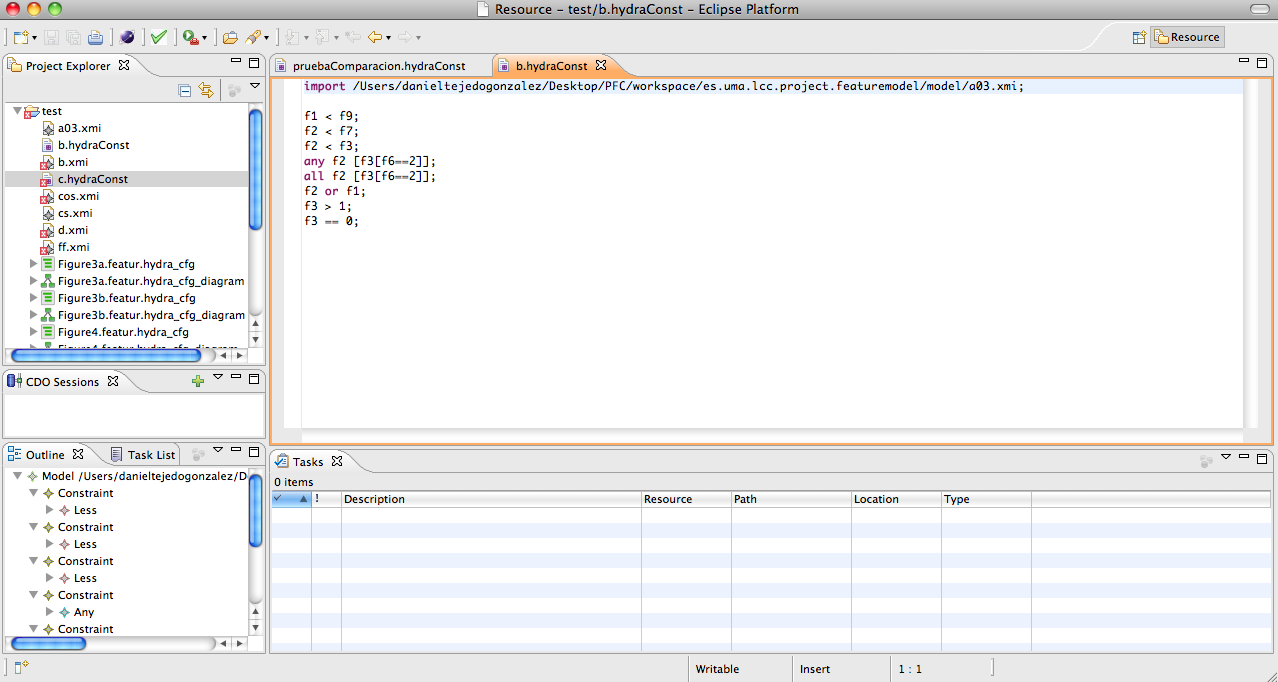
\includegraphics[scale=0.34]{semantica/editor.eps}
    \caption{Interfaz gr�fica del editor para el lenguaje HCL}
    \label{figeditor}
\end{figure}

Tras la implementaci�n de este bot�n, se comprob� su correcto funcionamiento mediante diversas pruebas, proporcion�ndole, por ejemplo, ficheros de configuraci�n tanto v�lidos e inv�lidos. Tras esto, se concluy� la implementaci�n del editor para el lenguaje \emph{Hydra Constraint Language}, pudiendo proceder a su empaquetado y distribuci�n.

%%=============================================================================%%
%% NOTA(Pablo): Esta figura sobra. Se�ala el bot�n sobre la otra imagen        %%  
%%=============================================================================%%
%%
%% \begin{figure}[t]
%%      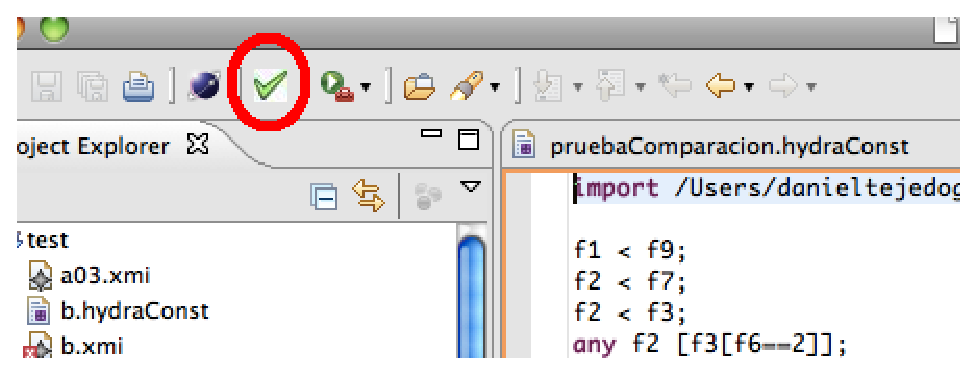
\includegraphics[scale=0.74]{semantica/boton.eps}
%%      \caption{Bot�n que ejecutar� la validaci�n de las restricciones}
%%      \label{figboton}
%% \end{figure}
%% 
%%=============================================================================%%

